\noindent Giả sử các cạnh song song với dây dẫn có chiều dài là $a$, các cạnh còn lại có chiều dài là $b$. Chọn trục $Ox$ như hình vẽ, gọi $x$ là toạ độ của cạnh gần nhất của khung so với dây dẫn, tại thời điểm ban đầu, khoảng cách này bằng $x_{0}$. Giả sử dòng điện trong dây dẫn có cường độ $I$, khi đó, cảm ứng từ do dây dẫn tạo ra ở khoảng cách $r$ là:
\begin{equation*}
  B(I,r)=\frac{\mu_{0}I}{2\pi r}
\end{equation*}
trong đó, $\mu_{0}$ là độ từ thẩm trong chân không. \\

\begin{figure}[h]
  \centering
  \begin{subfigure}[b]{0.49\textwidth}
    \centering
    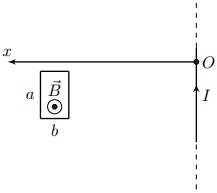
\includegraphics[width=0.65\textwidth]{Figures/Fig 4S1.jpg}
  \end{subfigure}
  \hfill
  \begin{subfigure}[b]{0.49\textwidth}
    \centering
    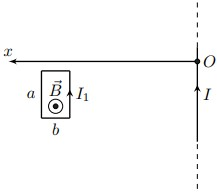
\includegraphics[width=0.65\textwidth]{Figures/Fig 4S2.jpg}
  \end{subfigure}
\end{figure}

\noindent Gọi dòng điện cảm ứng trong khung có cường độ $I_{1}$ và có hướng ngược chiều kim đồng hồ. Lực tác dụng lên khung dây là:
\begin{equation*}
  F_{x}=I_{1}aB(I,x+b)-I_{1}aB(I,x)
\end{equation*}
vì $a,b\ll x_{0}$, ta có:
\begin{equation*}
  F_{x}\approx\frac{\mu_{0}I_{1}Ia}{2\pi}\frac{d}{dx}\left(\frac{1}{x}\right)b=-\frac{\mu_{0}I_{1}Iab}{2\pi x^{2}}
\end{equation*}
gọi $R$ là điện trở của khung và $\phi$ là thông lượng từ qua khung, theo định luật Faraday:
\begin{equation*}
  I_{1}=-\frac{\dot{\phi}}{R}
\end{equation*}
vì kích thước của khung dây rất nhỏ so với khoảng cách từ nó đến dây dẫn, ta có thể xem cảm ứng từ là không đổi trên toàn bộ diện tích của khung dây, khi đó từ thông là:
\begin{equation*}
  \phi\approx B(x)ab
\end{equation*}
suy ra:
\begin{equation*}
  I_{1}=-\frac{ab}{R}\frac{dB(x)}{dt}=-\frac{\mu_{0}ab}{2\pi R}\frac{d}{dt}\left(\frac{I}{x}\right)
\end{equation*}
do đó:
\begin{equation*}
  F_{x}=\left(\frac{\mu_{0}ab}{2\pi}\right)^{2}\frac{I}{R}\frac{1}{x^{2}}\frac{d}{dt}\left(\frac{I}{x}\right)
\end{equation*}
vì cường độ dòng điện trong dây dẫn tăng lên rất nhanh, ta có thể bỏ qua chuyển động của khung trong thời gian tăng dòng điện, khi đó:
\begin{equation*}
  F_{x}\approx\left(\frac{\mu_{0}ab}{2\pi}\right)^{2}\frac{I}{Rx^{3}}\frac{dI}{dt}
\end{equation*}
gọi $m$ và $v_{x}$ lần lượt là khối lượng và vận tốc của khung trên phương $x$, ta có:
\begin{equation*}
  m\frac{dv_{x}}{dt}=\left(\frac{\mu_{0}ab}{2\pi}\right)\frac{I}{Rx^{3}}\frac{dI}{dt}
\end{equation*}
suy ra:
\begin{equation*}
  mdv_{x}=\left(\frac{\mu_{0}ab}{2\pi}\right)\frac{IdI}{Rx^{3}}
\end{equation*}
tích phân hai vế ta được:
\begin{equation*}
  mv_{0}=\left(\frac{\mu_{0}abI_{0}}{2\pi}\right)^{2}\frac{1}{2Rx_{0}^{3}}
\end{equation*}
bây giờ, ta sẽ xem xét chuyển động tiếp theo của khung, khi cường độ dòng điện trong dây dẫn đạt giá trị không đổi $I_{0}$, lực tác dụng lên khung là:
\begin{equation*}
  F_{x}=\left(\frac{\mu_{0}abI_{0}}{2\pi}\right)^{2}\frac{1}{Rx^{2}}\frac{d}{dx}\left(\frac{1}{x}\right)=-\left(\frac{\mu_{0}abI_{0}}{2\pi}\right)^{2}\frac{1}{Rx^{4}}\frac{dx}{dt}
\end{equation*}
định luật II Newton:
\begin{equation*}
  m\frac{dv_{x}}{dt}=-\left(\frac{\mu_{0}abI_{0}}{2\pi}\right)^{2}\frac{1}{Rx^{4}}\frac{dx}{dt}
\end{equation*}
suy ra:
\begin{equation*}
  mdv_{x}=-\left(\frac{\mu_{0}abI_{0}}{2\pi}\right)^{2}\frac{dx}{Rx^{4}}
\end{equation*}
tích phân hai vế ta được:
\begin{equation*}
  m(v_{1}-v_{0})=-\frac{2mv_{0}}{3}\implies v_{1}=\frac{v_{0}}{3}
\end{equation*}
vì $v_{1}>0$, khung sẽ chuyển động ra xa dây dẫn, do đó, nó sẽ không bao giờ dừng lại.\\
